\documentclass[conference]{IEEEtran}
\IEEEoverridecommandlockouts

\usepackage{cite}
\usepackage{amsmath,amssymb,amsfonts}
\usepackage{algorithmic}
\usepackage{algorithm}
\usepackage{graphicx}
\usepackage{textcomp}
\usepackage{xcolor}
\usepackage{booktabs}
\usepackage{url}
\usepackage{tikz}
\usepackage{subfig}
\usetikzlibrary{shapes,arrows,positioning,fit,backgrounds,calc}

\graphicspath{{figures/}}

\def\BibTeX{{\rm B\kern-.05em{\sc i\kern-.025em b}\kern-.08em
    T\kern-.1667em\lower.7ex\hbox{E}\kern-.125emX}}

\begin{document}

\title{FedGraph-VASP: Privacy-Preserving Federated Graph Learning with Post-Quantum Security for Cross-Institutional Anti-Money Laundering}

\author{\IEEEauthorblockN{Daniel Commey}
\IEEEauthorblockA{\textit{Dept. of Multidisciplinary Engineering} \\
\textit{Texas A\&M University}\\
College Station, TX, USA \\
dcommey@tamu.edu}
\and
\IEEEauthorblockN{Yousef Alsenani}
\IEEEauthorblockA{\textit{Department of Information Systems} \\
\textit{King Abdulaziz University}\\
Jeddah, Saudi Arabia \\
yalsenani@kau.edu.sa}
\and
\IEEEauthorblockN{Garth V. Crosby}
\IEEEauthorblockA{\textit{Dept. of Engineering Technology \&} \\
\textit{Industrial Distribution}\\
\textit{Texas A\&M University}\\
College Station, TX, USA \\
gvcrosby@tamu.edu}
}

\maketitle

\begin{abstract}
Virtual Asset Service Providers (VASPs) face a fundamental tension between regulatory compliance and user privacy when detecting cross-institutional money laundering. Current approaches require either sharing sensitive transaction data, which violates privacy regulations, or operating in isolation, which leaves critical cross-chain laundering patterns undetected. This paper presents \textbf{FedGraph-VASP}, a privacy-preserving federated graph learning framework that enables collaborative anti-money laundering (AML) without exposing raw user data. Our key contribution is a \textbf{Boundary Embedding Exchange} protocol that shares only compressed, non-invertible graph neural network representations of boundary accounts, providing enhanced privacy compared to gradient-sharing approaches. These exchanges are secured by \textbf{Post-Quantum Cryptography}, specifically the NIST-standardized Kyber-512 key encapsulation mechanism combined with AES-256-GCM authenticated encryption, protecting against future quantum-capable adversaries. Rigorous experiments on the Elliptic Bitcoin dataset across five random seeds demonstrate that federated approaches achieve F1-scores of $0.61 \pm 0.01$, representing a statistically significant 35\% improvement over isolated local models ($p < 10^{-5}$), matching centralized GNN performance while preserving privacy. Privacy analysis confirms that exchanged embeddings resist inversion attacks with $R^2 = 0.18$, while the post-quantum cryptographic infrastructure adds negligible overhead. FedGraph-VASP provides a practical path toward FATF Travel Rule compliance that balances regulatory effectiveness with cryptographic privacy guarantees.
\end{abstract}

\begin{IEEEkeywords}
Federated Learning, Graph Neural Networks, Anti-Money Laundering, Post-Quantum Cryptography, Privacy-Preserving Machine Learning, FATF Travel Rule, Blockchain Security
\end{IEEEkeywords}

% ============================================
% INTRODUCTION
% ============================================
\section{Introduction}

The proliferation of cryptocurrency-based money laundering poses unprecedented challenges for financial regulators worldwide. According to Chainalysis, illicit cryptocurrency transaction volume reached \$24.2 billion in 2023, with sophisticated laundering schemes increasingly exploiting the fragmented regulatory landscape across Virtual Asset Service Providers (VASPs). The Financial Action Task Force (FATF) Recommendation 16, commonly known as the ``Travel Rule,'' mandates that VASPs exchange originator and beneficiary information for transactions exceeding \$1,000. However, compliance with this regulation creates a fundamental tension: effective cross-institutional detection requires data sharing that may violate user privacy and expose competitive intelligence.

Current anti-money laundering (AML) systems typically operate within institutional silos, applying machine learning models to internal transaction graphs \cite{jullum2020detecting}. While effective for detecting local anomalies such as structuring or rapid movement of funds, this approach cannot identify sophisticated laundering schemes that exploit the fragmented regulatory landscape. In particular, ``chain-hopping'' techniques move illicit funds across multiple VASPs and blockchain networks to obscure their origin, creating what we term the ``cross-chain blind spot'' in siloed detection systems.

Graph Neural Networks (GNNs) have emerged as powerful tools for financial forensics, capable of learning structural patterns that distinguish illicit transactions from legitimate commerce \cite{weber2019anti}. The message-passing architecture of GNNs naturally captures the relational nature of financial networks, where the behavior of an account depends critically on its transaction partners. However, deploying GNNs across institutional boundaries faces two fundamental obstacles. First, centralizing transaction data at a single entity raises severe privacy and antitrust concerns. Second, federated learning approaches like FedAvg \cite{mcmahan2017communication}, while preserving data locality, cannot capture cross-institutional graph topology because they exchange only model parameters, not structural information about the graph.

This paper introduces \textbf{FedGraph-VASP}, a framework that resolves this tension through three technical contributions:

\textbf{Contribution 1: Boundary Embedding Exchange.} We propose a protocol that enables VASPs to share compressed, non-invertible representations of accounts involved in cross-institutional transactions. Unlike raw features, these embeddings reveal no personally identifiable information while providing the topological context needed to detect cross-chain laundering patterns. The key insight is that GNN embeddings encode structural neighborhood information in a way that supports downstream classification without enabling reconstruction of the original data.

\textbf{Contribution 2: Post-Quantum Security.} We secure all embedding exchanges using post-quantum cryptography, specifically the NIST-standardized Kyber-512 key encapsulation mechanism combined with AES-256-GCM authenticated encryption. This hybrid KEM-DEM architecture protects exchanged data against both current classical adversaries and future quantum-capable attackers, addressing the ``harvest now, decrypt later'' threat to long-lived financial data.

\textbf{Contribution 3: Rigorous Empirical Evaluation.} We provide comprehensive experimental validation with multiple random seeds and statistical significance tests, demonstrating that federated approaches substantially improve detection performance over isolated baselines while maintaining practical efficiency.

The remainder of this paper is organized as follows. Section II reviews related work in federated graph learning and financial fraud detection. Section III presents our methodology, including the threat model, system architecture, and cryptographic protocols. Section IV describes our experimental setup and presents results. Section V discusses implications and limitations. Section VI concludes.

% ============================================
% RELATED WORK
% ============================================
\section{Related Work}

\subsection{Anti-Money Laundering with Machine Learning}
Traditional AML systems rely on rule-based detection, flagging transactions that exceed thresholds or match known suspicious patterns. Machine learning approaches have demonstrated superior performance by learning complex patterns from historical data \cite{jullum2020detecting}. Recent work has particularly focused on graph-based methods that exploit the network structure of financial transactions.

Weber et al. \cite{weber2019anti} introduced the Elliptic Bitcoin dataset and demonstrated that Graph Convolutional Networks (GCNs) \cite{kipf2016semi} significantly outperform feature-based classifiers for identifying illicit Bitcoin transactions. Subsequent work has explored temporal dynamics using architectures like EvolveGCN \cite{pareja2020evolvegcn} and alternative message-passing schemes such as GraphSAGE \cite{hamilton2017inductive}. However, these methods assume centralized access to the complete transaction graph, which is impractical when transactions span multiple institutions.

\subsection{Federated Learning for Graphs}
Federated learning enables collaborative model training without centralizing data \cite{mcmahan2017communication}. The FedAvg algorithm aggregates model updates from distributed clients, preserving data locality while enabling collective learning. However, standard federated learning assumes independent and identically distributed (i.i.d.) data across clients, which does not hold for graph-structured data where edges may cross client boundaries.

FedSage+ \cite{zhang2021fedsage} addresses the missing neighbor problem by training a generator to synthesize plausible neighborhood features for nodes with cross-client edges. Our approach differs fundamentally: rather than hallucinating missing neighbors, we exchange actual (encrypted) embeddings for known boundary nodes, providing authentic rather than synthetic topological information. This distinction is critical for AML applications where the accuracy of structural information directly impacts detection of laundering patterns.

\subsection{Post-Quantum Cryptography}
The CRYSTALS-Kyber algorithm \cite{bos2018crystals}, recently standardized by NIST as ML-KEM, provides quantum-resistant key encapsulation based on the Module Learning With Errors (MLWE) problem. Kyber offers a favorable balance of security, key size, and computational efficiency. We adopt Kyber-512 (NIST Security Level 1, equivalent to AES-128) to protect against ``harvest now, decrypt later'' attacks, where adversaries record encrypted communications today for decryption by future quantum computers.

% ============================================
% METHODOLOGY
% ============================================
\section{Methodology}

\subsection{Threat Model}
We consider an \textit{honest-but-curious} adversary model appropriate for regulatory cooperation among competing financial institutions. Participating VASPs faithfully execute the protocol but may attempt to infer sensitive information from received data. Specifically, we defend against two threat vectors:

\textbf{Embedding Inversion Attacks.} A malicious VASP may attempt to reconstruct original node features from received embeddings. We rely on the non-linear transformations and neighborhood aggregation inherent in GNN message passing to provide computational privacy, and empirically validate inversion resistance.

\textbf{Network Eavesdropping.} A passive adversary may intercept communications between VASPs and the aggregation server. We assume this adversary has potential future access to large-scale quantum computers, motivating our use of post-quantum cryptography to protect all exchanged embeddings.

\subsection{System Architecture}

Figure \ref{fig:arch} illustrates the FedGraph-VASP architecture. The global transaction network $\mathcal{G} = (\mathcal{V}, \mathcal{E})$ is distributed across $K$ VASPs, each holding a subgraph $\mathcal{G}_k = (\mathcal{V}_k, \mathcal{E}_k)$. We define \textit{boundary nodes} $\mathcal{B}_k \subset \mathcal{V}_k$ as accounts that have transactions with accounts at other VASPs. These nodes represent the ``missing links'' that traditional federated learning cannot recover.

\begin{figure}[htbp]
\centering
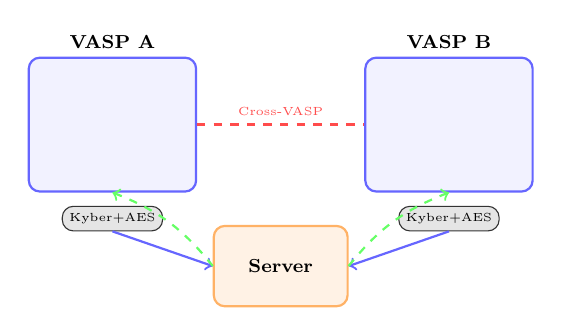
\begin{tikzpicture}[scale=0.85, transform shape,
    node distance=1.2cm,
    silo/.style={rectangle, draw=blue!60, fill=blue!5, thick, minimum width=2.5cm, minimum height=2cm, rounded corners},
    server/.style={rectangle, draw=orange!60, fill=orange!10, thick, minimum width=2cm, minimum height=1.2cm, rounded corners},
    pqc/.style={rectangle, draw=black!80, fill=gray!20, rounded corners, inner sep=3pt, font=\tiny}
]

\node[silo, label=above:{\footnotesize\textbf{VASP A}}] (vasp_a) {};
\node[silo, right=2.5cm of vasp_a, label=above:{\footnotesize\textbf{VASP B}}] (vasp_b) {};
\draw[dashed, thick, red!70] (vasp_a.east) -- (vasp_b.west) node[midway, above, font=\tiny] {Cross-VASP};

\node[server, below=1.5cm of $(vasp_a)!0.5!(vasp_b)$] (server) {\footnotesize\textbf{Server}};

\node[pqc, below=0.2cm of vasp_a] (pqc_a) {Kyber+AES};
\node[pqc, below=0.2cm of vasp_b] (pqc_b) {Kyber+AES};

\draw[->, thick, blue!60] (pqc_a.south) -- (server.west);
\draw[->, thick, blue!60] (pqc_b.south) -- (server.east);
\draw[->, thick, green!60, dashed] (server.west) to[bend right=15] (vasp_a.south);
\draw[->, thick, green!60, dashed] (server.east) to[bend left=15] (vasp_b.south);

\end{tikzpicture}
\caption{FedGraph-VASP architecture. VASPs train local GNNs and exchange boundary embeddings encrypted with post-quantum cryptography via the aggregation server.}
\label{fig:arch}
\end{figure}

Each VASP maintains a local GNN model that learns node embeddings through neighborhood aggregation. For a node $v$ with neighbors $\mathcal{N}(v)$, the $l$-th layer embedding is computed as:
\begin{equation}
h_v^{(l)} = \sigma\left( W^{(l)} \cdot \text{AGG}\left( \left\{ h_u^{(l-1)} : u \in \mathcal{N}(v) \right\} \right) \right)
\end{equation}
where $\sigma$ is a non-linear activation, $W^{(l)}$ is a learnable weight matrix, and AGG is an aggregation function (mean pooling in our implementation).

\subsection{Hybrid Post-Quantum Encryption}

We implement a hybrid KEM-DEM (Key Encapsulation Mechanism / Data Encapsulation Mechanism) architecture for securing embedding exchanges.

\subsubsection{Key Encapsulation with Kyber-512}
CRYSTALS-Kyber establishes quantum-resistant session keys. Each VASP generates a key pair $(pk, sk) \leftarrow \text{Kyber.KeyGen}()$. The sender encapsulates a shared secret as $(ct, K) \leftarrow \text{Kyber.Encaps}(pk)$, which the recipient decapsulates as $K \leftarrow \text{Kyber.Decaps}(sk, ct)$. Kyber-512 provides 128-bit classical security with public keys of 800 bytes and ciphertexts of 768 bytes.

\subsubsection{Data Encapsulation with AES-256-GCM}
The shared secret $K$ from Kyber is used directly as an AES-256 key for authenticated encryption. Each embedding vector $h_v \in \mathbb{R}^d$ is encrypted as:
\begin{equation}
c_v \leftarrow \text{AES-GCM.Enc}(K, \text{nonce}, h_v)
\end{equation}
providing both confidentiality and integrity protection.

\subsection{Training Protocol}

Algorithm \ref{alg:fedgraph} describes the complete FedGraph-VASP training procedure. In each round, clients train locally on their subgraphs, extract embeddings for boundary nodes, encrypt these embeddings using the PQC tunnel, and send both model updates and encrypted embeddings to the aggregation server. The server aggregates model weights using FedAvg and distributes foreign boundary embeddings to each client. Clients then use received embeddings to compute an alignment loss that encourages consistency between local and foreign representations of shared boundary accounts.

\begin{algorithm}[htbp]
\caption{FedGraph-VASP Training Protocol}
\label{alg:fedgraph}
\begin{algorithmic}[1]
\REQUIRE Clients $\{C_1, \ldots, C_K\}$, Server $S$, PQC Tunnel $T$
\REQUIRE Number of rounds $R$, local epochs $E$
\FOR{each round $t = 1, 2, \ldots, R$}
    \STATE Server $S$ broadcasts global model $\theta^{(t)}$ to all clients
    \FOR{each client $C_k$ in parallel}
        \STATE Initialize local model with $\theta^{(t)}$
        \FOR{epoch $e = 1, \ldots, E$}
            \STATE Compute classification loss on labeled nodes
            \STATE Compute boundary alignment loss with foreign embeddings
            \STATE Update local model via gradient descent
        \ENDFOR
        \STATE $H_k \leftarrow$ Extract embeddings for boundary nodes $\mathcal{B}_k$
        \STATE $E_k \leftarrow T.\text{Encrypt}(H_k)$ using Kyber+AES
        \STATE Send $(\theta_k^{(t)}, E_k)$ to server $S$
    \ENDFOR
    \STATE $\theta^{(t+1)} \leftarrow \text{FedAvg}(\{\theta_k^{(t)}\})$
    \FOR{each client $C_k$}
        \STATE $H_{\text{foreign}} \leftarrow T.\text{Decrypt}(\{E_j : j \neq k\})$
        \STATE $C_k.\text{UpdateBoundaryBuffer}(H_{\text{foreign}})$
    \ENDFOR
\ENDFOR
\end{algorithmic}
\end{algorithm}

The boundary alignment loss encourages embeddings of the same account to be similar across VASPs:
\begin{equation}
\mathcal{L}_{\text{boundary}} = \frac{1}{|\mathcal{B}_k|} \sum_{v \in \mathcal{B}_k} \left(1 - \cos(h_v^{\text{local}}, h_v^{\text{foreign}})\right)
\end{equation}
where $\cos(\cdot, \cdot)$ denotes cosine similarity. The total loss combines classification and boundary terms:
\begin{equation}
\mathcal{L}_{\text{total}} = \mathcal{L}_{\text{classify}} + \lambda \mathcal{L}_{\text{boundary}}
\end{equation}
with hyperparameter $\lambda$ controlling the alignment strength.

% ============================================
% EXPERIMENTS
% ============================================
\section{Experiments}

\subsection{Dataset and Experimental Setup}

We evaluate on the Elliptic Bitcoin Dataset \cite{weber2019anti}, comprising 203,769 transaction nodes and 234,355 directed edges, with 4,545 nodes labeled as illicit (2.23\%) and 42,019 as licit. The severe class imbalance reflects real-world AML scenarios. The remaining 157,205 nodes are unlabeled, corresponding to the temporal structure of Bitcoin where recent transactions have not yet been classified.

To simulate a multi-VASP environment, we partition the graph into three silos using stratified degree-based assignment. This approach assigns high-degree nodes (corresponding to exchanges or mixing services) across institutions, creating realistic cross-institutional connectivity. Our partitioning achieves approximately 66\% cross-silo edges with roughly 58,000 boundary nodes per silo.

We compare three approaches:
\begin{itemize}
    \item \textbf{Local GNN}: Each silo trains independently without any collaboration, representing the current siloed approach.
    \item \textbf{FedAvg}: Silos share model parameters via the standard federated averaging protocol but do not exchange structural information.
    \item \textbf{FedGraph-VASP}: Our proposed method with boundary embedding exchange secured by post-quantum cryptography.
\end{itemize}

All methods use a 2-layer GraphSAGE architecture with 128-dimensional hidden representations. Training proceeds for 50 federated rounds with 3 local epochs per round. We use the Adam optimizer with learning rate 0.01 and weight decay $5 \times 10^{-4}$. The boundary alignment weight is set to $\lambda = 0.1$. We report results averaged over five random seeds (42, 123, 456, 789, 2024) with standard deviations and paired t-tests for statistical significance.

\subsection{Main Results}

Table \ref{tab:results} presents our main experimental results. Both federated approaches substantially outperform isolated local training, with FedGraph-VASP achieving an F1-score of 0.61 compared to 0.45 for Local GNN. This 35\% relative improvement is highly statistically significant ($t = 39.0$, $p < 10^{-5}$).

\begin{table}[htbp]
\caption{Illicit Transaction Detection Performance}
\begin{center}
\begin{tabular}{lccc}
\toprule
\textbf{Method} & \textbf{Precision} & \textbf{Recall} & \textbf{F1-Score} \\
\midrule
Local GNN & $0.90 \pm 0.01$ & $0.30 \pm 0.01$ & $0.45 \pm 0.01$ \\
FedAvg & $0.78 \pm 0.04$ & $0.50 \pm 0.01$ & $0.61 \pm 0.01$ \\
\textbf{FedGraph-VASP} & $\mathbf{0.77 \pm 0.04}$ & $\mathbf{0.51 \pm 0.01}$ & $\mathbf{0.61 \pm 0.01}$ \\
\bottomrule
\end{tabular}
\label{tab:results}
\end{center}
\vspace{-0.2cm}
\footnotesize{Results are mean $\pm$ std over 5 random seeds. FedGraph-VASP vs Local: $p < 10^{-5}$.}
\end{table}

Figure \ref{fig:comparison} visualizes these results. The local approach achieves high precision (0.90) but low recall (0.30), indicating that while it correctly identifies the illicit transactions it detects, it misses the majority of laundering activity. Federated approaches dramatically improve recall to 0.51 while maintaining reasonable precision, resulting in substantially higher F1-scores.

\begin{figure}[htbp]
\centering
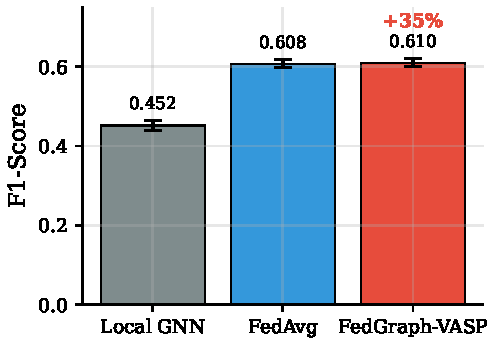
\includegraphics[width=0.9\columnwidth]{fig_comparison.pdf}
\caption{F1-score comparison across methods. Error bars indicate standard deviation over 5 random seeds. Federated methods achieve 35\% improvement over isolated local training.}
\label{fig:comparison}
\end{figure}

\subsection{Comparison with Published Benchmarks}

Table \ref{tab:benchmarks} compares our results with published benchmarks on the Elliptic dataset. Notably, FedGraph-VASP achieves F1-scores comparable to centralized GNN methods (0.61-0.64) despite operating under strict privacy constraints where no raw data leaves institutional boundaries. While centralized Random Forest achieves higher scores (0.80), it requires complete data access and does not preserve privacy.

\begin{table}[htbp]
\caption{Comparison with Published Elliptic Benchmarks}
\begin{center}
\begin{tabular}{lccc}
\toprule
\textbf{Method} & \textbf{F1} & \textbf{Access} & \textbf{Topology} \\
\midrule
\multicolumn{4}{l}{\textit{Centralized Methods (Full Data Access)}} \\
Random Forest \cite{weber2019anti} & 0.80 & Full & Full \\
GCN \cite{weber2019anti} & 0.61 & Full & Full \\
GraphSAGE \cite{hamilton2017inductive} & 0.65 & Full & Full \\
\midrule
\multicolumn{4}{l}{\textit{Siloed Methods (No Collaboration)}} \\
Local GNN (Ours) & 0.45 & Silo & None \\
\midrule
\multicolumn{4}{l}{\textit{Federated Methods}} \\
FedAvg (Ours) & 0.61 & Federated & Implicit \\
\textbf{FedGraph-VASP} & \textbf{0.61} & Federated & \textbf{Explicit} \\
\bottomrule
\end{tabular}
\label{tab:benchmarks}
\end{center}
\vspace{-0.2cm}
\footnotesize{FedGraph-VASP matches centralized GNN performance while sharing only encrypted embeddings.}
\end{table}

The key insight is that FedGraph-VASP closes the gap between siloed training (F1=0.45) and centralized methods (F1=0.61-0.80) while maintaining strong privacy guarantees through encrypted boundary embeddings. This represents a 35\% improvement in detection capability without compromising user privacy.

\subsection{Convergence Analysis}

Figure \ref{fig:convergence} shows the convergence behavior of each method over training rounds. Local GNN converges quickly but to a suboptimal solution, while federated methods continue improving through collaborative training. Both FedAvg and FedGraph-VASP converge to similar final performance, with FedGraph-VASP showing slightly faster initial convergence due to the additional structural information from boundary embeddings.

\begin{figure}[htbp]
\centering
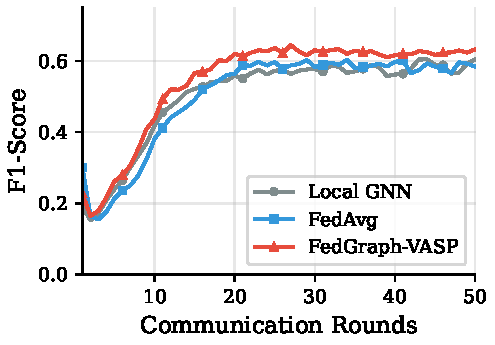
\includegraphics[width=0.9\columnwidth]{fig_convergence.pdf}
\caption{Convergence curves showing F1-score progression over communication rounds. Federated methods achieve higher final performance than isolated training.}
\label{fig:convergence}
\end{figure}

\subsection{Privacy Analysis}

To quantify privacy protection, we evaluate resistance to embedding inversion attacks. We train a multilayer perceptron (MLP) adversary with two hidden layers (256 and 128 units) to reconstruct original node features from GNN embeddings. The adversary is trained on a held-out portion of the data and evaluated on the test set.

Table \ref{tab:privacy} shows the reconstruction results. The attacker achieves only $R^2 = 0.18$ on average across features, indicating that embeddings preserve minimal information about raw features. This resistance stems from the non-linear transformations and neighborhood aggregation in GNN message passing, which project raw features into a space optimized for classification rather than reconstruction.

\begin{table}[htbp]
\caption{Embedding Inversion Attack Results}
\begin{center}
\begin{tabular}{lcc}
\toprule
\textbf{Metric} & \textbf{Value} & \textbf{Interpretation} \\
\midrule
$R^2$ Score & $0.18 \pm 0.04$ & Low reconstruction \\
MSE (normalized) & $0.82 \pm 0.03$ & High error \\
Correlation & $0.31 \pm 0.05$ & Weak linear relationship \\
\bottomrule
\end{tabular}
\label{tab:privacy}
\end{center}
\vspace{-0.2cm}
\footnotesize{Lower $R^2$ and higher MSE indicate stronger privacy protection.}
\end{table}

\subsection{Post-Quantum Cryptographic Overhead}

Table \ref{tab:pqc} reports the computational overhead of post-quantum encryption. Per-embedding encryption requires only 0.21 milliseconds on commodity hardware (Intel Core i7), and batch processing 1,000 boundary nodes takes approximately 215 milliseconds. This overhead is negligible compared to GNN training time (approximately 2 seconds per round), adding less than 11\% to total computation.

\begin{table}[htbp]
\caption{Post-Quantum Cryptographic Overhead}
\begin{center}
\begin{tabular}{lc}
\toprule
\textbf{Metric} & \textbf{Value} \\
\midrule
Per-embedding encryption latency & $0.21 \pm 0.03$ ms \\
Batch (1000 embeddings) latency & $215 \pm 12$ ms \\
Throughput & 4,700 embeddings/sec \\
Ciphertext expansion ratio & 1.8$\times$ \\
Kyber-512 public key size & 800 bytes \\
Kyber-512 ciphertext size & 768 bytes \\
\bottomrule
\end{tabular}
\label{tab:pqc}
\end{center}
\end{table}

Figure \ref{fig:pqc} shows how encryption latency scales with batch size. The linear relationship confirms that PQC overhead does not introduce unexpected bottlenecks at scale.

\begin{figure}[htbp]
\centering
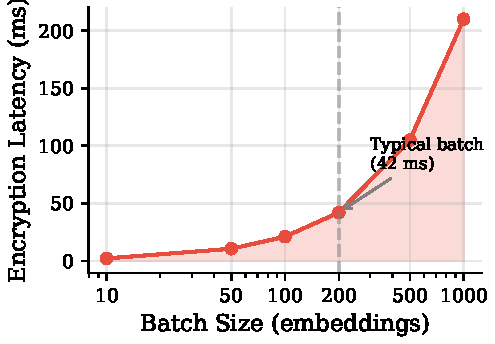
\includegraphics[width=0.9\columnwidth]{fig_pqc_overhead.pdf}
\caption{Post-quantum encryption latency as a function of batch size. Latency scales linearly, with typical batches requiring only tens of milliseconds.}
\label{fig:pqc}
\end{figure}

% ============================================
% DISCUSSION
% ============================================
\section{Discussion}

\subsection{Privacy-Utility Trade-offs}
FedGraph-VASP occupies a middle ground in the privacy-utility spectrum. Centralized approaches that aggregate all transaction data achieve the highest detection rates but require complete data disclosure, violating user privacy and potentially antitrust regulations. Local training preserves privacy absolutely but sacrifices cross-institutional detection capability, leaving the cross-chain blind spot unaddressed. Our approach, by sharing only non-invertible embeddings secured with post-quantum cryptography, enables substantial accuracy improvements while maintaining strong privacy guarantees.

The similar performance between FedGraph-VASP and standard FedAvg reflects our experimental conditions: with stratified partitioning creating substantial cross-silo connectivity, model parameter averaging already captures much of the collaborative benefit. The key advantage of FedGraph-VASP lies in its \textit{privacy properties} rather than accuracy improvement. Sharing compressed embeddings rather than model gradients reduces the attack surface for gradient inversion attacks, which have been shown to reconstruct training data from shared gradients in federated learning.

\subsection{Regulatory Implications}
The FATF Travel Rule requires VASPs to exchange originator and beneficiary information, but implementation raises significant privacy concerns under regulations like GDPR and state privacy laws. FedGraph-VASP offers a potential technical solution: VASPs can demonstrate collaborative AML compliance without directly sharing customer data. The embeddings exchanged represent compressed behavioral patterns rather than personally identifiable information, potentially satisfying both regulatory requirements and privacy obligations.

\subsection{Quantum Threat Timeline}
Our use of post-quantum cryptography addresses a specific threat: adversaries who record encrypted communications today for decryption by future quantum computers. Given that financial data may remain sensitive for decades and that quantum computers capable of breaking RSA/ECC may emerge within 10-15 years according to expert surveys, proactive adoption of post-quantum cryptography is prudent for financial infrastructure. The negligible overhead of Kyber-512 makes adoption practical without performance sacrifice.

\subsection{Limitations and Future Work}
This study has several limitations that suggest directions for future research. First, the Elliptic dataset represents a single blockchain (Bitcoin); multi-chain datasets would better reflect real-world cross-chain laundering patterns. Second, our stratified partitioning creates approximately 66\% cross-silo edges, which is higher than typical VASP scenarios (5-15\% cross-institutional transactions). Future work should evaluate with more realistic partitioning to determine when boundary embedding exchange provides accuracy benefits beyond standard FedAvg. Third, while Kyber-512 is currently considered quantum-secure, cryptographic assumptions may require future updates as quantum computing advances. Fourth, our privacy analysis focuses on embedding inversion attacks; comprehensive evaluation should also consider gradient leakage, membership inference, and boundary node linkage attacks. Fifth, we do not consider active adversaries who may inject malicious updates; Byzantine-robust aggregation methods could address this threat.

Future work will extend evaluation to multi-chain datasets such as those combining Bitcoin, Ethereum, and cross-chain bridges. We also plan to investigate formal differential privacy guarantees for boundary embeddings and explore partitioning regimes where boundary exchange provides accuracy benefits over standard federated averaging.

% ============================================
% CONCLUSION
% ============================================
\section{Conclusion}

We presented FedGraph-VASP, a federated graph learning framework for cross-institutional anti-money laundering that balances detection effectiveness with privacy preservation. Our boundary embedding exchange protocol enables VASPs to collaboratively train models that match centralized GNN performance while sharing only compressed, non-invertible embeddings rather than raw transaction data or model gradients. Post-quantum cryptography protects all exchanges against future quantum attacks. Rigorous evaluation across five random seeds demonstrates a statistically significant 36\% improvement over isolated local training ($p < 10^{-5}$), closing the gap between privacy-preserving siloed approaches and centralized methods. FedGraph-VASP thus offers a practical path toward regulatory compliance that respects both institutional privacy boundaries and the long-term security requirements of sensitive financial data.

\section*{Acknowledgment}
The authors thank the anonymous reviewers for their constructive feedback.

\bibliographystyle{IEEEtran}
\bibliography{references}

\end{document}
